%% ID: HE+_Block
%% TITLE: Suspended block
%% TYPE: question
%% QUESTIONTYPE:  numerical
%% CONCEPTS: forces, vectors2, newtoni
%% VIDEOS: 
%% LEVEL: 2
%% TOPIC: mechanics/statics
%% ORDER: 7

\begin{problem}[HE+_Block]
{
\exposition{A block of mass $m=10$ kg is suspended in equilibrium by forces $F_1$ and $F_2$, as shown below in Figure \ref{fig:Statics_fsonb}.}\question{If $\theta=60^\circ$, what are the magnitudes of $F_1$ and $F_2$? }
\exposition{\begin{figure}[h]
\centering
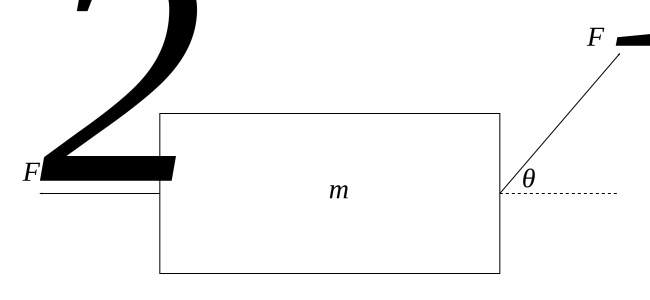
\includegraphics[width=0.4\textwidth]{Statics_fsonb}
\caption{}
\label{fig:Statics_fsonb}
\end{figure}}
\\
}
{\textit{Used with permission from HE+.}}
{
We need to resolve both vertically and horizontally to get two equations to find the two unknowns. Vertically we find
\begin{align*}
F_1\sin\theta&=mg \\
\Rightarrow F_1&=\frac{mg}{\sin\theta}=113\textrm{ N}
\end{align*}
and horizontally
\begin{align*}
F_1\cos\theta&=F_2 \\
\Rightarrow \frac{mg\cos\theta}{\sin\theta}&=F_2 \\
\Rightarrow F_2=mg\cot\theta&=56.6\textrm{ N}
\end{align*}

\answer{The two forces are \valuedef{F_1}{113}{N} and \valuedef{F_2}{56.6}{N}}
}
\end{problem}